\documentclass[reprint,nofootinbib,amsmath,amssymb,aps,floatfix]{revtex4-2}

\usepackage[utf8]{inputenc}
\usepackage{graphicx}
\usepackage{bm}
\usepackage{booktabs}
\usepackage{placeins}
\usepackage{hyperref}
\hypersetup{colorlinks=true, linkcolor=blue!55!black, citecolor=blue!55!black, urlcolor=blue!55!black}
\usepackage{microtype}
\usepackage{mathtools}
\usepackage{xcolor}
\renewcommand{\thefigure}{\arabic{figure}}
\newcommand{\logA}{\ensuremath{\log A}\xspace}
\usepackage{xspace}

\begin{document}

\title{Frequentist, Bayesian and machine-learning analysis of the stiffness of resistant breast-cancer cells from AFM force curves}

\author{Giacomo Moretti}
\affiliation{Università degli Studi di Milano-Bicocca}

\begin{abstract}
We analyse 257 AFM force--distance curves measured on the cytoplasm and on the nucleus of two resistant breast-carcinoma
lines (MCF7R and T47DR). Each curve is reduced to the effective elastic parameter $A$ of a Hertz-like model,
$F=A\,\delta^{3/2}$, and the distributions of $\log A$ are compared between regions with the same statistical
toolbox in a frequentist (profile likelihood, toy Monte Carlo, Holm correction, systematics), a Bayesian (MCMC, Bayes
factors, hierarchical model) and a machine-learning (anomaly detection with injected defects, classification,
mixtures) setting. The nucleus is softer than the cytoplasm in both lines: $\Delta=\mu_{nucleus}-\mu_{cytoplasm}=-0.81\pm0.08$
(MCF7R) and $-0.25\pm0.10$ (T47DR) in $\log A$, i.e.\ a ratio of typical $A$ of 0.44 and 0.78. The evidence is overwhelming for MCF7R and
only weak for T47DR (Bayes factor $\sim4{:}1$ despite $p\simeq0.01$). The analysis is limited by pseudo-replication
and by the coincidence of cell line and measurement session.
\end{abstract}

\maketitle

\section{Introduction}
Cell stiffness measured by atomic force microscopy (AFM) is a label-free marker of cell state, and of the response of
tumour cells to treatment. The aim of this work is to compare the mechanical properties of two resistant
breast-carcinoma lines, MCF7R and T47DR, in two measurement regions (cytoplasm and nucleus) at 48~h, starting from raw
force--distance curves. The emphasis is on the \emph{statistical} treatment: every comparison is made with explicit
models, its behaviour is validated with toy Monte Carlo experiments, and the dependence on analysis choices is
quantified. The pipeline is implemented in five notebooks (reading and QC, contact point and fit, frequentist,
Bayesian and machine-learning analysis; see Sec.~\ref{sec:code}).

\section{Data and curve reduction}\label{sec:data}
The data are 257 JPK force files in four groups: MCF7R cytoplasm (55 curves), MCF7R nucleus (60), T47DR cytoplasm (59)
and T47DR nucleus (83), measured with an MLCT-BIO triangular cantilever (spring constant $\simeq0.12$~N/m). Each file
holds an extend (approach) and a retract segment; the extend segment is used for the mechanical fit, the retract one for
the adhesion. The curves are the «good curves» already selected by the experimenters; a preliminary instrumental QC
(robust $z$-scores of noise, force excursion and jumps) is computed but \emph{no curve is discarded}.

For each extend curve the baseline is a robust line fitted on the first 30\% of the points (the tip is far from the
surface), the noise $\sigma_b$ is the MAD of its residuals, and the contact point is initialised where the smoothed force exceeds
$\max(8\sigma_b,\,5\%F_{max})$ for 20 consecutive points. In the window $0.08F_{max}<F<0.8F_{max}$ the data are fitted with
\begin{equation}
F(\delta)=A\,\delta^{3/2},\qquad \delta=z_c-z,
\end{equation}
with $A$ and the contact point $z_c$ free~\cite{hertz1882}. The tip radius and the Poisson ratio are not available, so $A$ is an
\emph{effective} parameter in nN\,$\mu$m$^{-3/2}$ and not the Young modulus; the MLCT-BIO tip is pyramidal, for which a
Sneddon-type model~\cite{sneddon1965} with exponent 2 would apply, so only \emph{relative} comparisons are meaningful. The fits
have median $R^2=0.986$ and a relative statistical error on $A$ of 0.8\%, far smaller than the spread of $A$ between curves
(Sec.~\ref{sec:freq}), which is therefore intrinsic. Figure~\ref{fig:fit} shows one fit.
$A$ is positive and right-skewed, so the analysis uses $\log A$ (with $A$ in nN\,$\mu$m$^{-3/2}$).

\begin{figure}[tb]
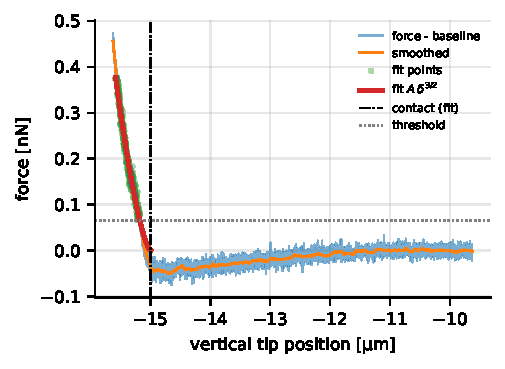
\includegraphics[width=\columnwidth]{figures/fit_example.pdf}
\caption{Example of baseline-corrected curve, contact point and Hertz-like fit (MCF7R cytoplasm).}\label{fig:fit}
\end{figure}

\section{Statistical model}
In each group $g$ we model $x_i=\log A_i\sim\mathcal N(\mu_g,\sigma_g^2)$ (a log-normal $A$). Figure~\ref{fig:groups} shows the
distributions: the Gaussian is adequate for the bulk, and $\log A$ is much more symmetric than $A$ (skewness of $A$ from 0.8 to 3.1, of $\log A$ from $-0.2$ to 0.9; the largest values are in the nucleus groups, see Sec.~\ref{sec:disc-skew}).
The parameter of interest is the nucleus--cytoplasm shift $\Delta_l=\mu_{l,nucleus}-\mu_{l,cytoplasm}$ for each line $l$;
$e^{\Delta}$ is the ratio of the typical $A$, and $\Delta<0$ means a softer nucleus.

\begin{figure}[tb]
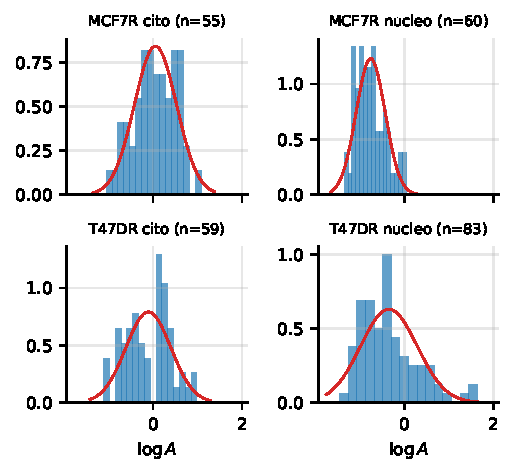
\includegraphics[width=\columnwidth]{figures/logA_groups.pdf}
\caption{Distribution of $\log A$ in the four groups with the fitted Gaussian.}\label{fig:groups}
\end{figure}

\section{Frequentist analysis}\label{sec:freq}
\textbf{Estimation.} The parameters are obtained from the unbinned likelihood with \texttt{iminuit}~\cite{iminuit}; Hesse and Minos
errors coincide with the analytic $\sigma/\sqrt n$ (e.g.\ MCF7R nucleus: $\hat\mu=-0.757\pm0.042$, $\hat\sigma=0.325\pm0.030$).

\textbf{Profile likelihood.} For fixed $\Delta$ the maximisation over the other parameters is analytic up to $\mu_{cytoplasm}$, so the
profile is computed exactly. The 68\% intervals and the Wilks test~\cite{wilks1938} give
$\Delta_{\mathrm{MCF7R}}=-0.814\,^{+0.077}_{-0.076}$ ($q=70.7$, $p<10^{-15}$) and
$\Delta_{\mathrm{T47DR}}=-0.247\,^{+0.096}_{-0.095}$ ($q=6.5$, $p=0.011$). Welch, Mann--Whitney, permutation and bootstrap-of-medians
tests agree (T47DR: $p=0.011$, $0.003$, $0.015$; median difference $-0.27$, 95\% interval $[-0.67,-0.07]$), so the conclusion does
not depend on the Gaussian assumption.

\textbf{Toy Monte Carlo validation.} Generating $1500$ experiments per line from the fitted model, the estimator is unbiased
(bias $<10^{-3}$), the pulls have mean 0.01 and width 0.98--1.00, the 68\% intervals cover $0.680$ and $0.679$, and the size at the
nominal 5\% is $0.059$ (MCF7R) and $0.052$ (T47DR), equal to Welch and Mann--Whitney. The power at the real sample size is 1.00
for MCF7R and $0.73$ for T47DR; 80\% power requires $|\Delta|\gtrsim0.22$--$0.25$, so T47DR sits just below the sensitivity threshold (Fig.~\ref{fig:toys}).

\begin{figure}[tb]
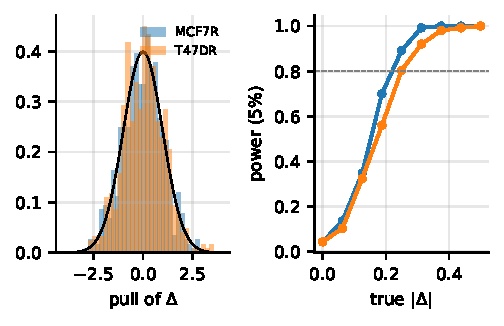
\includegraphics[width=\columnwidth]{figures/toys.pdf}
\caption{Toy Monte Carlo of the profile-likelihood estimator. Left: pull of $\Delta$ (black: standard normal). Right: power of the Wilks test versus the true $|\Delta|$.}\label{fig:toys}
\end{figure}

\textbf{Interaction and multiple tests.} A nested test of the additive model $\mu_{l,r}=a_l+b_r$ against the full model rejects it
($q=20.6$, $p=6\cdot10^{-6}$): the nucleus effect depends on the line. Between lines, $\Delta_{\text{T47DR--MCF7R}}$ is $-0.16\pm0.09$ in the cytoplasm
and $+0.41\pm0.08$ in the nucleus; however the two lines were measured on different days, so this comparison is confounded with the session. The four
confirmatory tests after Holm correction have $p=2\cdot10^{-16}$, $0.021$ (T47DR nucleus--cytoplasm), $0.089$ and $5\cdot10^{-6}$.

\textbf{Systematics.} Nine variants change one preprocessing choice at a time (baseline fraction, threshold, lower and upper
fit-window edge). With the Barlow criterion~\cite{barlow2002} no variant is significant for MCF7R and the total systematic is
$0.07$ for T47DR, smaller than its statistical error $0.10$ (Fig.~\ref{fig:bf}, right).

\section{Bayesian analysis}
\textbf{Model and sampling.} The same model with weakly informative priors ($\mu_g\sim\mathcal N(0,1)$, $\sigma_g\sim$ HalfNormal(1)) is sampled
with \texttt{emcee}~\cite{emcee} (40 walkers; $\hat R_{max}<1.03$, integrated autocorrelation time $\lesssim100$ steps). The posteriors of
$\Delta$ (median, 68\% interval) are $-0.81\,[-0.89,-0.74]$ and $-0.25\,[-0.34,-0.14]$, with $P(\Delta<0)=1.00$ and $0.993$; they coincide
with the profile intervals and are stable under wide, narrow and Jeffreys priors (shifts $\le0.03$).

\textbf{Bayes factors.} Marginalising $\sigma$ analytically, the evidence of $H_1$ ($\Delta\sim\mathcal N(0,\tau^2)$) against $H_0$ ($\Delta=0$) is
computed by exact numerical integration. For MCF7R $\log_{10}BF_{10}\simeq14$ for any $\tau\gtrsim0.3$. For T47DR $\log_{10}BF_{10}\le0.8$ (about 6:1 at best,
$0.6$ at $\tau=0.5$) and negative for $\tau\gtrsim5$ (Fig.~\ref{fig:bf}, left): a small effect that $p\simeq0.01$ would call significant is only weak
evidence in the Bayesian sense~\cite{kass1995}.

\textbf{Model checks.}\label{sec:disc-skew} A Student-$t$ likelihood is not preferred (WAIC~\cite{waic} difference $-0.4$, $\nu\simeq39$), so heavy tails are not the problem. The
posterior predictive check reproduces mean and standard deviation in all groups but not the \emph{skewness} of the nucleus groups (T47DR nucleus: $p_{PPC}\simeq0$;
MCF7R nucleus: $0.04$; Fig.~\ref{fig:ppc}). The chains are well mixed (Fig.~\ref{fig:ppc}, left).

\textbf{Hierarchical model.} Writing $\mu_{l,nucleus}=a_l+b+u_l$ with $u_l\sim\mathcal N(0,\tau_u^2)$, the common effect is
$b=-0.49\,[-0.77,-0.16]$ and $\tau_u=0.43\,[0.26,0.71]$, confirming that the effect differs between lines. Partial pooling moves the line effects by less than $0.03$.

\textbf{Low statistics.} With $5$--$80$ curves per group, the 68\% credible interval over-covers slightly (0.72 at $n=5$, 0.68 at $n=80$) and the profile interval under-covers (0.62 at
$n=5$, 0.66 at $n=80$), at the price of intervals longer by 30\% at $n=5$; the two agree for $n\gtrsim20$.

\begin{figure}[tb]
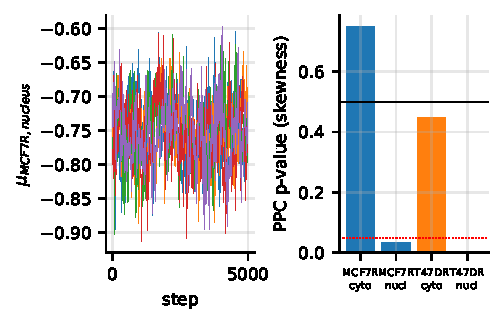
\includegraphics[width=\columnwidth]{figures/mcmc_ppc.pdf}
\caption{Left: trace of $\mu_{MCF7R,nucleus}$ for five walkers. Right: posterior predictive $p$-value of the skewness in each group (dotted: $0.05$).}\label{fig:ppc}
\end{figure}

\begin{figure}[tb]
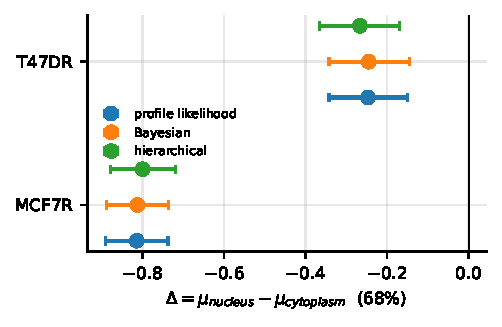
\includegraphics[width=\columnwidth]{figures/delta_methods.pdf}
\caption{$\Delta$ (nucleus -- cytoplasm) in $\log A$ with the three methods.}\label{fig:delta}
\end{figure}

\begin{figure}[tb]
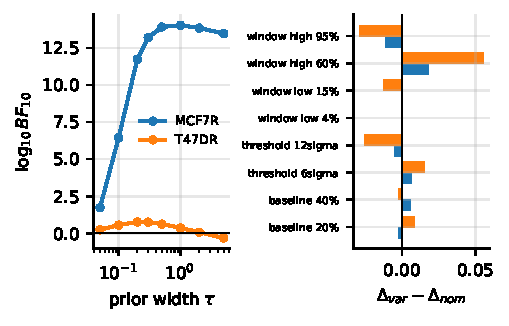
\includegraphics[width=\columnwidth]{figures/bf_systematics.pdf}
\caption{Left: Bayes factor versus the prior width on $\Delta$. Right: shift of $\Delta$ for each preprocessing variant.}\label{fig:bf}
\end{figure}

\section{Machine learning}
\textbf{Anomaly detection with known truth.} Since all real curves are pre-selected, the efficiency of anomaly detection is measured on 1000 synthetic Hertz-like
curves whose parameters are sampled from the real fits (including a correlated model mismatch), with 5\% of injected defects
(\texttt{no\_contact}, \texttt{saturation}, \texttt{huge\_noise}, \texttt{jump}, \texttt{wrong\_slope}). Isolation Forest~\cite{liu2008} and a robust
Mahalanobis distance, both unsupervised and trained only on good curves, reach AUC $0.88$ and $0.87$; at a 5\% false-positive rate the efficiencies are 100\% for
\texttt{no\_contact} and \texttt{huge\_noise} (these already fail the fit), $60$--$90\%$ for \texttt{saturation} and \texttt{jump}, and only $10$--$30\%$ for \texttt{wrong\_slope}
(Fig.~\ref{fig:ml}, left; 10 defects per type, i.e.\ about $\pm15\%$). Applied to the real curves (trained on them, cross-validated), the detector flags 8 curves in common with the
second detector, for visual inspection only.

\textbf{Classification of the region.} From $\log A$, maximum indentation and two adhesion features, a logistic model separates nucleus and cytoplasm with
AUC $0.95$ in MCF7R and $0.63$ in T47DR (cross-validated; permutation tests $p=0.005$ and $0.025$), consistent with the effects of the previous sections
(Figs.~\ref{fig:ml}, right, and~\ref{fig:roc}). Trained on one line and tested on the other, the AUC is $0.66$ (MCF7R$\to$T47DR) and $0.96$ (T47DR$\to$MCF7R): the sign of the effect is shared, its size is not.

\begin{figure}[tb]
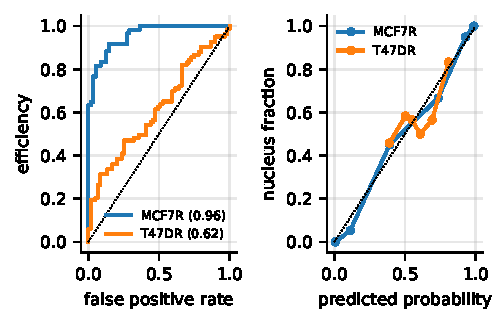
\includegraphics[width=\columnwidth]{figures/roc_calibration.pdf}
\caption{Cross-validated ROC (AUC in the legend) and calibration of the logistic nucleus/cytoplasm classifier.}\label{fig:roc}
\end{figure}

\textbf{Mixtures.} A parametric-bootstrap likelihood-ratio test favours two Gaussian components only for T47DR nucleus ($p=0.010$; $71\%$ at $\log A=-0.64$ and $29\%$ at $0.35$);
this is the origin of the skewness seen in the posterior predictive check.

\begin{figure}[tb]
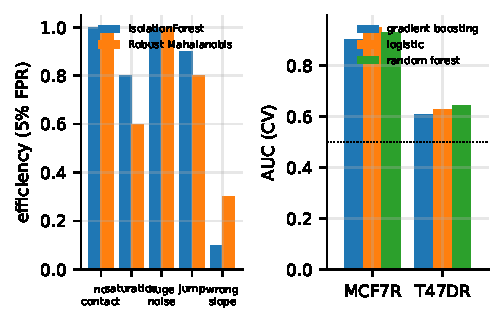
\includegraphics[width=\columnwidth]{figures/ml.pdf}
\caption{Left: anomaly-detection efficiency on synthetic defects. Right: cross-validated AUC of the nucleus/cytoplasm classifiers.}\label{fig:ml}
\end{figure}

\section{Discussion and limits}
The three approaches agree on the size of the effect and differ only in how they weigh the evidence for T47DR, which is the honest summary: the nucleus of MCF7R is clearly softer than its
cytoplasm ($\times0.44$ in $A$), while for T47DR the effect ($\times0.78$) is indicative and below the 80\%-power threshold at the available sample size.
The main limits are:
(i) \textbf{pseudo-replication}: several curves come from the same cell and the cell identifier is not available, so the errors are optimistic; a hierarchical model with cell as grouping factor is the natural extension;
(ii) \textbf{cell line $\equiv$ session}: the lines were measured on different days (25/02 and 18/03), so differences between lines cannot be separated from session effects;
(iii) \textbf{pre-selected sample}: no real defects are available, so the efficiency of the anomaly detection is optimistic;
(iv) \textbf{effective parameter}: $A$ is not the Young modulus and assumes a 3/2 exponent;
(v) the high-$A$ tail of T47DR nucleus suggests subpopulations, which a comparison of means does not describe.

\section{Code}\label{sec:code}
All results are produced by five notebooks in \texttt{Code\_General/} (\texttt{01} reading and QC, \texttt{02} contact point and fit, \texttt{03} frequentist, \texttt{04} Bayesian,
\texttt{05} machine learning) and the shared module \texttt{afm\_tools.py}; the figures are regenerated by \texttt{Docs/report/make\_figures.py} from \texttt{Code\_General/results/}.
The raw data are not distributed with the repository (see the README).

\appendix
\section{Notation and formulas}\label{app:notation}
\textbf{Quantities.} $A$: effective elastic parameter (nN\,$\mu$m$^{-3/2}$); $x=\log A$; $\mu_{l,r},\sigma_{l,r}$: mean and standard deviation of $x$ for
line $l\in\{$MCF7R, T47DR$\}$ and region $r\in\{$cytoplasm, nucleus$\}$; $\Delta_l=\mu_{l,nucleus}-\mu_{l,cytoplasm}$; $e^{\Delta}$: ratio of typical $A$.

\textbf{Profile likelihood.} With $n_c,n_n$ curves and $S_c(\mu)=\sum_i(x_i-\mu)^2$ over the cytoplasm curves, $S_n(\mu,\Delta)=\sum_j(x_j-\mu-\Delta)^2$ over the nucleus curves,
profiling $\sigma_c^2=S_c/n_c$ and $\sigma_n^2=S_n/n_n$ gives
\begin{equation}
-2\ln\mathcal L_{\rm prof}(\Delta)=\min_{\mu}\left[n_c\ln\frac{S_c(\mu)}{n_c}+n_n\ln\frac{S_n(\mu,\Delta)}{n_n}\right]+\text{const.},
\end{equation}
and the 68\% interval is where this rises by one unit above its minimum; the test of $\Delta=0$ uses $q=-2\ln\mathcal L_{\rm prof}(0)+2\ln\mathcal L_{\rm prof}(\hat\Delta)\sim\chi^2_1$.

\textbf{Bayes factor.} With the improper prior $p(\sigma)\propto1/\sigma$ common to both hypotheses, integrating $\sigma_c,\sigma_n$ out gives
\begin{equation}
p(\text{data}\mid\mu,\Delta)\propto S_c(\mu)^{-n_c/2}\,S_n(\mu,\Delta)^{-n_n/2},
\end{equation}
and $BF_{10}=\iint p(\text{data}\mid\mu,\Delta)\,\mathcal N(\mu;0,1)\,\mathcal N(\Delta;0,\tau^2)\,d\mu\,d\Delta\,/\!\int p(\text{data}\mid\mu,0)\,\mathcal N(\mu;0,1)\,d\mu$,
evaluated on a grid.

\textbf{Barlow criterion.} A variant with estimates $\Delta_v$ and error $\sigma_v$ gives a significant shift if $|\Delta_v-\Delta_{nom}|/\sqrt{|\sigma_v^2-\sigma_{nom}^2|}>2$.

\textbf{Anomaly score and efficiency.} The anomaly score is minus the Isolation Forest score (or the robust Mahalanobis distance); the threshold is the 95th percentile of the cross-validated scores of good
training curves, so the false-positive rate is 5\% by construction; the efficiency of a defect type is the fraction of defective curves above threshold, counting failed fits as detected.

\bibliography{biblio}

\end{document}
